Our aim is to show that the agents controlling an industrial micro-grid can learn complex behaviors and coordination strategies that can lead to an optimization of the global energy consumption. Therefore, we train the agents in different competitive and cooperative scenarios. In each scenario, the environment consists of multiples agents with discrete action space, discrete time space and mixed observation spaces. Every agent controls a grid component and may take physical actions in the environment by changing the operational state of the corresponding grid component. We do not assume that all agents have identical action and observation spaces, or act according to the same policy $\pi_{\theta}$. The environment of each experiment were implemented as an extension of OpenAI environment Gym \cite{Brockman01540}. We found this framework useful for creating environments involving complex interaction between agents, while keeping the control and perception problems simple, as we are primarily interested in addressing agent strategies. 

Unless otherwise specified, the actor and the critic of each agent is parameterized by a two-layer ReLU MLP with respectively $256$ units per layer for the actor and $512$ units per layer for the critic. In all of our experiments, we use the Adam optimizer with a learning rate of $0.0001$ and the discount factor $\gamma$ is set to be $0.9$. The size of the replay buffer is $10240$ and the sampling time horizon is $1024$. We update the network parameters after every $1024$ sampling steps and we use a batch size of $512$. We train with $10$ random seeds for environments with stark success/fail conditions (\textit{experiment 2} and \textit{experiment 3}) and with only $2$ seed for \textit{experiment 1}. For the PPO-algorithm, we set the clipping parameter $\epsilon$ to $0.1$, the entropy coefficient to $0.005$ and the exploration noise to $0.2$.

This section describes in details the designed experiments as well as the specific training parameters and analyzes various aspects of the learned behaviors. Codes for the environments as well as learned policy parameters of the agents in all environments are open-sourced and available at \cite{Bakakeu2019}.

\subsection{Experiment 1: Auto-Curricula and Emergent Behavior}
\label{subsec:51}
In this scenario, we consider a micro-grid of $4$ identical production machines (energy loads) executing the same production task. The grid is operated in connected mode. However, the main grid can only provide enough energy for $3$ production machines to operate. Therefore, the production machines are in full competition. The exploration reward of the agents is set so that the agent is penalized if the production machine is shouted down or suspended. The competition reward is based on the performance of the machines meaning that the agent will receive a positive incentive every time a production task is accomplished. In addition, all agents are penalized if the total energy demand is greater than the energy provided by the main grid. The exploration annealing factor $\alpha$ is set to $0.2$ so that the agent will first learn how to execute a production task during the initial $20\%$ of the training time. During the training each agent observed the full environment including the observations and the actions of the other agents. During the execution, the agents only observe the amount of energy available as well as the current operational state of the machine it controls. We train the agents with $2$ random seeds for $500$ sampling horizons.

% For figures use
%
\begin{figure}[b]
\sidecaption
% Use the relevant command for your figure-insertion program
% to insert the figure file.
% For example, with the graphicx style use
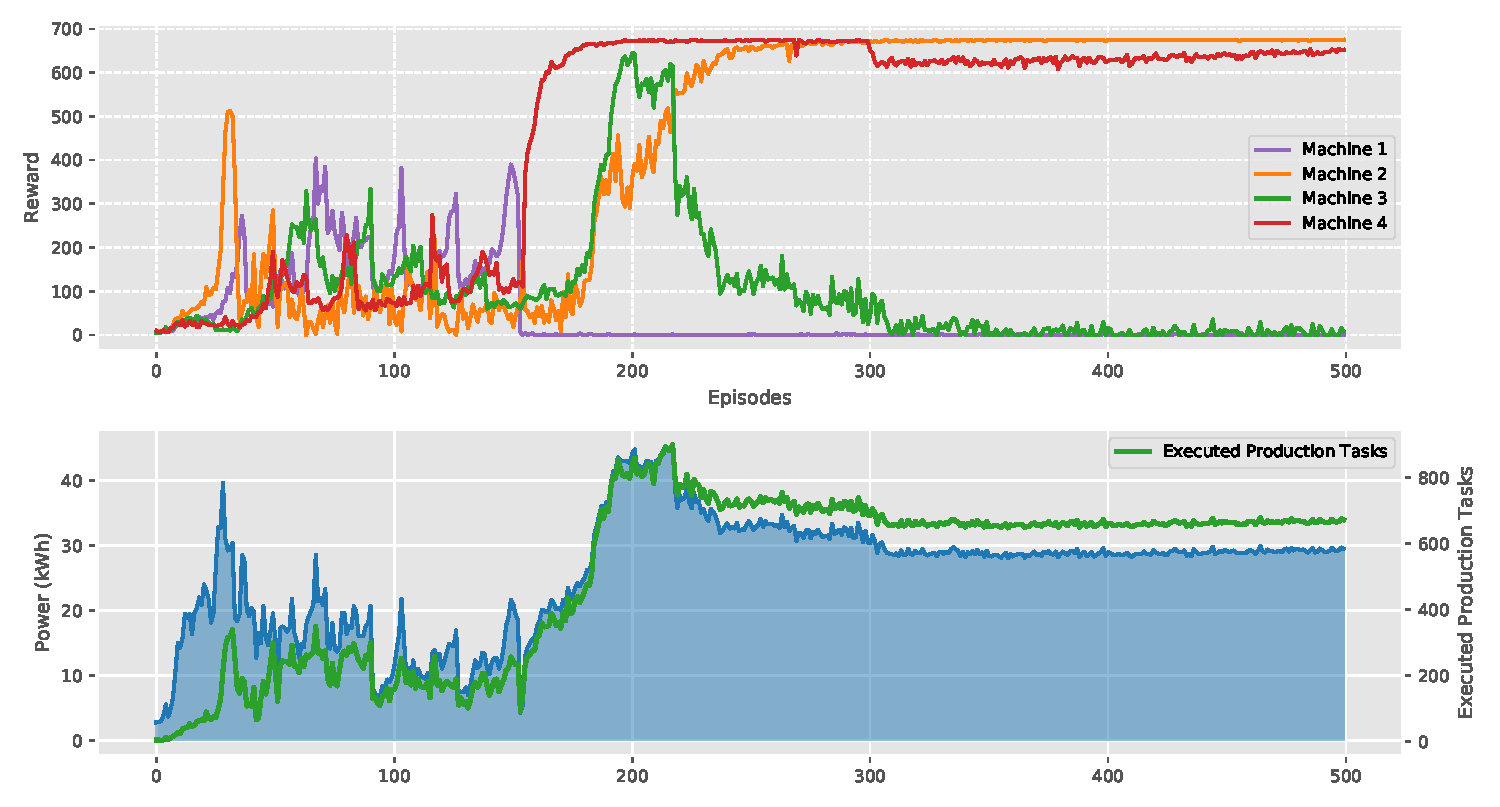
\includegraphics[scale=.48]{images/experiment_1_results}
%
% If no graphics program available, insert a blank space i.e. use
%\picplace{5cm}{2cm} % Give the correct figure height and width in cm
%
\caption{Emergent Skill Progression From Multi-Agent Autocurricula. Through the reward signal
agents go through different distinct stages of emergence. (a) Episode 1-30: the different agents learn basic skills (how to execute a production task) and the productivity rise. (b) Episode 30-160: strategy exploitation and competition take place between the agents and stabilize only when \textit{machine 1} adopts a very bad strategy. (c) Episode 160-220: the first coordination strategy emerge. \textit{Machine 2}, \textit{Machine 3} and \textit{Machine 4} start to produce more frequently while \textit{Machine 1} remains in the $idle$-state more often. (d) Episode 220-500: a second coordination strategy emerge.  \textit{Machine 2}, \textit{Machine 4} reached their highest productivity while \textit{Machine 3} is frequently halted.}
\label{fig:scenario_1_results}       % Give a unique label
\end{figure}

Fig. \ref{fig:scenario_1_results} shows a typical progression of the emergent strategies learned by all agents during the course of the training measured in this case by the respective average cumulative rewards. Clearly, training the agents against each other creates many different strategies, each of which introduces a previously non-existent pressure on other agents to do better in order to move to the next stage. Note that there are no direct incentives for agents to explore, but rather the emergent strategies are solely a result of the auto-curriculum induced by multi-agent competition.

Fig. \ref{fig:scenario_1_results} shows a typical progression of the emergent strategies. Initially, the agents learn simultaneously how to control the corresponding production machine so that it can reach the $execute$-state as often as possible. After approximately 30 episodes, all agent have mastered this task and the energy demand of the whole grid begin to surpass the energy provided by the main grid. Consequently, the agents are then frequently penalized leading to a significant reduction of the production performance and the accumulated reward. At this point some agents begin to take advantage of the observations and actions of other agents and intentionally modify their policies accordingly. We can see , for example, some agents wait in the $idle$-state and then switch to the $execute$-state, when other agents are stopped or halted. However, the more the new strategy becomes efficient, the more it becomes predictable and the other agents begin to defend themselves against this strategy. After another 5-20 episodes, all agents have now learned to exploit the strategy of other agents and the energy demand of the production machines again surpass the energy supply and the agents are penalized again more frequently. At this point a new adaptation/exploitation cycle restarts. Because of random exploration factors, the best performing agent during this phase changes from cycle to cycle. After approximately 3-6 cycles (which corresponds to episode 30 - 160), the training stabilized when at least one agent adopts a very bad policy e.g. only switching between $stopped$- and $idle$- state. The first acceptable coordination strategy emerges from episode 160 to approximately episode 220: \textit{Machine 2}, \textit{Machine 3} and \textit{Machine 4} start to produce more frequently while \textit{Machine 1} remains in the $idle$-state oftenly. It is a valid strategy since the energy required for the production can be supplied by the main grid and the overall productivity is  relatively high. The second and final coordination strategy emerge at episode 220: while \textit{Machine 2} and \textit{Machine 4} reached their highest productivity,  \textit{Machine 3} is frequently halted.

In this experiment, we found that the emergent auto-curriculum is fairly robust, as similar observations can be made with different initialization strategies. Out of $10$ experimental runs, more than $7$ runs were able to converge to an equilibrium. However, many design choices can drastically reduce the convergence time and the sample complexity such as the surrogate loss and the entropy loss of the underlying PPO-algorithm. We also experimented with different configurations (for example by including energy storage and generator components) and found that these configurations also lead to emergent behaviors, providing further evidence that multi-agent interaction is a promising path towards self-supervised energy management.

\subsection{Experiment 2: Fully Cooperative Production}
\label{subsec:52}

% For figures use
%
\begin{figure}[h!]
\sidecaption
% Use the relevant command for your figure-insertion program
% to insert the figure file.
% For example, with the graphicx style use
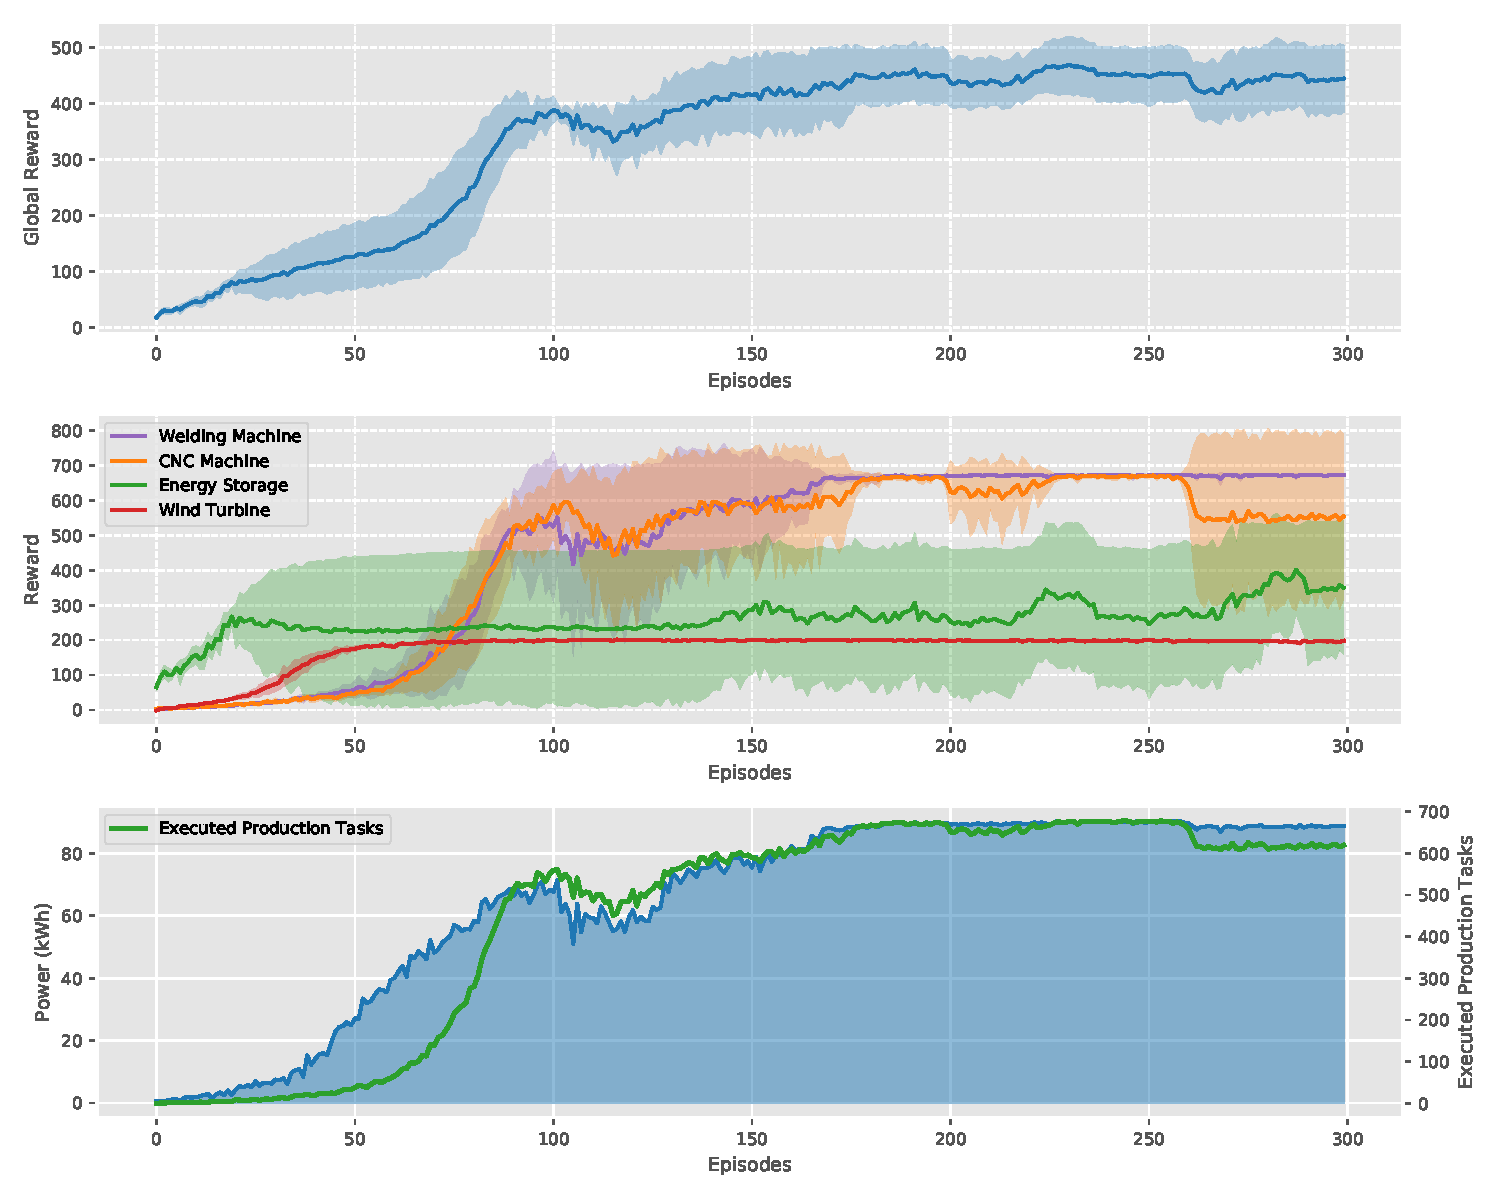
\includegraphics[scale=.48]{images/experiment_2_results}
%
% If no graphics program available, insert a blank space i.e. use
%\picplace{5cm}{2cm} % Give the correct figure height and width in cm
%
\caption{Average rewards on cooperative production. A coordination strategy emerges rapidly after $100$ episodes. While the energy generators rapidly learn how to generate energy, the energy storage component adopted to discharge when the production machines in the $execute$-state and thus allowing the production machine to increase the productivity.}
\label{fig:scenario_2_results}       % Give a unique label
\end{figure}

In this scenario, the micro-grid is operated in isolated mode and consists of two production machines (a CNC-machine and a welding machine), an energy generator (a wind turbine) and an energy storage system. The energy generated by the wind turbine is lower than the energy needed by the production machines. Therefore, the energy storage system has to be turned on in order to execute a production task. All the components should therefore cooperate. The exploration rewards is similar to the previous experiment and the team-based cooperation reward of the agents is based on the performance of the production machines. We train the agents for $300$ episodes. The agents also used the same policy network architecture as in experiment 1 (see section \ref{subsec:51}).

As we can observe in Fig. \ref{fig:scenario_2_results}, the components rapidly learn the required basic skills and a coordination strategy emerge around the episode $100$. While the energy generator is constantly switched on, the energy storage component learns to charge when the production machines are standing still and to discharge when the production machines perform a production task and thus supports production. Once the energy generator and the energy storage component have adopted a strategy, the production machines rapidly learn to increase their productivity which reach its highest level around episode $250$.

To determine the seed dependence of the skill emergence, we ran this environment with $10$ random seeds and looked at the variability of the onset of behavioral shifts across runs. We find that the behavioral shifts happen at very similar times around episode $100$ in training. Rewards and environment statistics are very consistent in early as well as in later times in training.

\subsection{Experiment 3: Effect of Exploration Curriculum}
\label{subsec:53}
... yet to come!!! [TODO: Jupiter Bakakeu]
